\documentclass[lineno]{jfm}

\usepackage{subcaption}
\usepackage{acro}

%%%%%%%%%% additional definitions %%%%%%%%%%
\newcommand\dstar{{\delta^*}} % displacement thickness
\newcommand\awave{{\alpha_\mathrm{p}}} % wavenumber of the primary (2D) wave in the secondary stability analysis
\DeclareMathOperator{\argmax}{arg\,max}

% acronyms
\DeclareAcronym{BFS}{short=BFS, long=backward-facing step}
\DeclareAcronym{FFS}{short=FFS, long=forward-facing step}
\DeclareAcronym{LSA}{short=LSA, long=linear stability analysis}
\DeclareAcronym{DNS}{short=DNS, long=direct numerical simulation}
\DeclareAcronym{TS}{short=TS, long=Tollmien--Schlichting}
%%%%%%%%%%%%%%%%%%%%%%%%%%%%%%%%%%%%%%%%%%%%

\lefttitle{V. Ballester Ribó, J. D. Crouch, Y. Hwang and S. J. Sherwin}
\righttitle{Journal of Fluid Mechanics}

\title{Secondary instability of the two-dimensional waves shed by surface gaps in incompressible boundary layers}

\author{Víctor Ballester Ribó\aff{1}, Jeffrey D. Crouch\aff{2}, Yongyun Hwang\aff{1} \and Spencer J. Sherwin\aff{1}}

\affiliation{\aff{1}Department of Aeronautics, Imperial College London, South Kensington, London SW7 2AZ, UK
\aff{2}The Boeing Company, P.O. Box 3707, Seattle, WA 98124-2207, USA}

\corresau{Víctor Ballester Ribó, \email{v.ballester-ribo24@imperial.ac.uk}}

\begin{document}
% lineno-FLM.sty (loaded by jfm.cls at \begin{document}) re-issues
% \newif\ifLineNumbers *after* \runninglinenumbers, which resets lineno's own
% flag to false and silently disables \linenomath.  The consequence is that the
% part of a paragraph preceding a display equation gets no line numbers.
\LineNumberstrue
\maketitle

\begin{abstract}
	TODO.
\end{abstract}

% Material moved from ../jfm_incNS/main.tex on 2026-11-09 (local secondary stability /
% local Floquet analysis of the 2D limit cycle). Cross-references to figures, equations
% and sections that stayed in the main paper (e.g. fig:3d2dDynamics1000,
% fig:freqUnstableMode, eq:amplitudeNorm, eq:3dperturbationEnergy) are left dangling.

\section{Formulation}\label{sec:numericalSetup}
The incompressible Navier--Stokes equations are solved using a spectral/\textit{hp}-element formulation. In nondimensional form, the governing equations are
\begin{equation}\label{eq:ns}
	\begin{aligned}
		\partial_t \boldsymbol{u} + (\boldsymbol{u}\cdot\bnabla)\,\boldsymbol{u} & = -\bnabla p + \frac{1}{\Rey} \nabla^2 \boldsymbol{u}, \\
		\bnabla \cdot \boldsymbol{u}                                       & = 0,
	\end{aligned}
\end{equation}
where $\boldsymbol{u}={(u_x,u_y,u_z)}^\mathrm{T}$ denotes the velocity field, $p$ is the pressure, and $\Rey$ is the Reynolds number. Throughout the paper, $\boldsymbol{x}={(x,y,z)}^\mathrm{T}$ denotes the Cartesian coordinates, with $x$, $y$ and $z$ denoting the streamwise, wall-normal and spanwise directions, respectively. The equations are nondimensionalised using the streamwise component of the free-stream velocity, $u_\infty$, as the characteristic velocity and the displacement thickness $\dstar$ as the characteristic length scale. The latter is evaluated at the upstream edge of the gap for the smooth-wall reference flow. Thus,
$
	\Rey \equiv \Rey_\dstar := u_\infty \dstar/\nu
$,
where $\nu$ is the kinematic viscosity of the flow. The Reynolds number is varied in the range $\Rey \in [800,3000]$. All the quantities in the paper are nondimensional unless otherwise stated.

For global \ac{LSA}, the Navier--Stokes equations~\eqref{eq:ns} are linearised around a base flow $\boldsymbol{Q}={(U_x,U_y,U_z,P)}^\mathrm{T}$, that is, a base velocity field $\boldsymbol{U}={(U_x,U_y,U_z)}^\mathrm{T}$ and a base pressure field $P$ that together solve~\eqref{eq:ns}. The base flows are obtained from nonlinear simulations of~\eqref{eq:ns} and they can be either an equilibrium solution for standard \ac{LSA} or a periodic orbit for Floquet analysis. When the base flow is globally unstable, the selective frequency damping method \citep{akervik2006,sfd} is used to suppress the unstable modes and obtain the corresponding unstable equilibrium solution. When the base flow is a stable periodic orbit, the periodic orbit is extracted through naive time integration. The state $\boldsymbol{q}={(u_x,u_y,u_z,p)}^\mathrm{T}$ is then decomposed as $\boldsymbol{q}=\boldsymbol{Q}+\boldsymbol{q}'$, where $\boldsymbol{q}'={(u_x',u_y',u_z',p')}^\mathrm{T}$ comprises the perturbation velocity field $\boldsymbol{u}'={(u_x',u_y',u_z')}^\mathrm{T}=\boldsymbol{u}-\boldsymbol{U}$ and the perturbation pressure $p'=p-P$. Substituting this decomposition into~\eqref{eq:ns} and retaining only the terms linear in $\boldsymbol{q}'$ gives the linearised equations, written in compact form as% chktex 8
\begin{equation}\label{eq:linearizedNS}
	\begin{aligned}
		\boldsymbol{\mathcal{M}}\partial_t\boldsymbol{q}'      & = \boldsymbol{\mathcal{L}}(\boldsymbol{U})\boldsymbol{q}',                                                                                                                                                   \\
		\qquad\qquad\boldsymbol{\mathcal{M}} = \begin{bmatrix}
			\boldsymbol{I}_3 & \boldsymbol{0} \\ \boldsymbol{0}^\mathrm{T} & 0 \end{bmatrix},\quad & \boldsymbol{\mathcal{L}}(\boldsymbol{U}) = \begin{bmatrix}
			-\mathcal{C}_{\boldsymbol{U}} + \frac{1}{\Rey}\nabla^2 & -\bnabla \\ \bnabla\cdot{} & 0
		                                                                                                                                    \end{bmatrix},
	\end{aligned}
\end{equation}
where $\boldsymbol{I}_3$ is the identity matrix of size 3 and $\mathcal{C}_{\boldsymbol{U}}\boldsymbol{u}':=(\boldsymbol{U}\cdot\bnabla)\,\boldsymbol{u}'+(\boldsymbol{u}'\cdot\bnabla)\,\boldsymbol{U}$ is the advection operator linearised around $\boldsymbol{U}$. For standard global \ac{LSA}, the base flow is constant in time. For Floquet analysis, the base flow depends on time and it is $T$-periodic, $\boldsymbol{U}(t+T)=\boldsymbol{U}(t)$. For this study, in both cases the base flow is independent of the spanwise coordinate, so perturbations separate into spanwise Fourier modes that evolve independently. Combining this with Floquet's theorem, solutions of~\eqref{eq:linearizedNS} are sought in the form
\begin{equation}\label{eq:floquetansatz}
	\boldsymbol{u}'(x,y,z,t)
	= \hat{\boldsymbol{u}}(x,y,t)\,\mathrm{e}^{\mathrm{i}\beta z}\,\mathrm{e}^{\lambda t},
	\qquad
	\hat{\boldsymbol{u}}(x,y,t+T)=\hat{\boldsymbol{u}}(x,y,t),
\end{equation}
where $\beta$ is the spanwise wavenumber and $\lambda$ is the complex Floquet exponent. For a spanwise-periodic domain of length $b$, the admissible wavenumbers are $\{\beta_k = 2\pi k/b : k=0,\ldots,15\}$. Throughout this paper, perturbations with $\beta=0$ are spanwise-uniform and are referred to as two-dimensional, whereas three-dimensional perturbations are those with $\beta\neq0$, which vary along the span. With this convention, the mode $k=0$, although trivially periodic in $z$, is not counted as three-dimensional. When the base flow is steady, $\hat{\boldsymbol{u}}$ is independent of time and~\eqref{eq:floquetansatz} reduces to the classical normal-mode ansatz. In both cases, the eigenvalue problem is solved with a matrix-free time-stepper approach \citep{tuckermanBarkley2000,barkleyBlackburnSherwin2008}. Integrating the linearised equations~\eqref{eq:linearizedNS} over a time interval $\tau$ defines the monodromy operator $\mathcal{A}(\tau)$, which maps an initial perturbation $\boldsymbol{q}'(0)$ onto $\boldsymbol{q}'(\tau)$. The eigenvalues $\mu$ of $\mathcal{A}(\tau)$ are related to the exponents $\lambda$ by $\mu=\mathrm{e}^{\lambda\tau}$, so that the eigenvalues of largest modulus correspond to the largest growth rates $\Re(\lambda)$. These leading eigenvalues and their eigenmodes are computed with an Arnoldi method that requires only repeated actions of $\mathcal{A}(\tau)$, that is, successive linearised simulations.

Local \ac{LSA} complements the global analysis and is used mainly to interpret the amplification of two-dimensional \ac{TS} waves across the gap. In this framework, the base flow is approximated as locally parallel at each streamwise location, $\boldsymbol{U}=(U(y;x),0)$, and perturbations are sought as normal modes of the form
\begin{equation}\label{eq:localansatz}
	\boldsymbol{u}'(x,y,z,t)
	=
	\hat{\boldsymbol{u}}(y)\,\mathrm{e}^{\mathrm{i}(\alpha x + \beta z - \omega t)},
\end{equation}
where $\alpha =\alpha_\mathrm{r}  + \mathrm{i}\alpha_\mathrm{i} $ is the complex streamwise wavenumber, $\beta $ the spanwise wavenumber and $\omega =\omega_\mathrm{r} +\mathrm{i}\omega_\mathrm{i} $ the complex frequency. Since \ac{TS} waves are two-dimensional, only $\beta=0$ is considered, and substituting~\eqref{eq:localansatz} into the linearised equations gives the Orr--Sommerfeld problem \citep{schmid2001stability}% chktex 8
\begin{equation}\label{eq:OS}
	{\big({\mathrm{D}}^2-{\alpha}^2\big)}^2\hat{u}_y
	-\mathrm{i}\Rey\left[
		(\alpha U-\omega)\big({\mathrm{D}}^2-{\alpha}^2\big)
		-\alpha U''\right]\hat{u}_y=0,
\end{equation}
for the wall-normal velocity component $\hat{u}_y$, where $\mathrm{D}:=\mathrm{d}/\mathrm{d}y$. The problem is subject to $\hat{u}_y(0)=\mathrm{D}\hat{u}_y(0)=0$ and $\hat{u}_y,\mathrm{D}\hat{u}_y\to0$ as $y\to\infty$. Fixing $\Rey$, the pairs $(\alpha,\omega)$ for which~\eqref{eq:OS} admits a non-trivial solution form the zero set of a dispersion function $\mathcal{D}(\alpha,\omega;\Rey)$. The temporal and spatial formulations are two different real restrictions of this same zero set: the temporal one prescribes $\alpha=\alpha_\mathrm{r}\in\mathbb{R}$ and solves for $\omega$, whereas the spatial one prescribes $\omega=\omega_\mathrm{r}\in\mathbb{R}$ and solves for $\alpha$. Equation~\eqref{eq:OS} is discretised by Chebyshev collocation on $81$ Gauss--Lobatto points, with the domain truncated at $y_{\max}=45$. The points are clustered near the wall by the algebraic mapping of \citet{malik1990}. Following \citet{bridgesMorris1984}, the auxiliary variable $\hat{q}=({\mathrm{D}}^2-\alpha^2)\hat{u}_y$ is introduced to reduce it to a quadratic problem in $\alpha$, which is then linearised into a generalised eigenvalue problem and solved with the QZ algorithm. Each streamwise station and frequency is solved independently, and the \ac{TS} mode is selected from the full spectrum as the least damped eigenvalue whose phase speed lies in $0.15<\omega_\mathrm{r}/\alpha_\mathrm{r}<0.75$.

To study how three-dimensional disturbances grow on the two-dimensional limit cycle, a local secondary stability analysis (local Floquet analysis) of the wave shed by the limit cycle, hereafter the primary wave, is performed along the lines of \citet{herbert1988}. It has three steps: a local model of the primary wave is built at each streamwise station from the two-dimensional simulations; the linear stability of this model to three-dimensional disturbances is posed as an eigenvalue problem for a temporal growth rate; and this rate is converted into a spatial growth rate, which can be compared with the streamwise growth of the three-dimensional disturbances in the simulations.

Downstream of the gap, the limit cycle is a wave of frequency $\omega$ travelling downstream. At a station $x_0$ it is approximated as locally parallel and periodic in $x$, with local wavenumber $\awave$, so that all its harmonics travel with the same phase speed $c=\omega/\awave$. The approximation requires the amplitude and the wavenumber of the wave to vary slowly over a wavelength, $2\pi/\awave\approx20$--$25$, which holds downstream of the gap as long as the wave is not decaying rapidly. In the frame moving with the wave, $\xi=x-ct$, the wave is then steady and $2\pi/\awave$-periodic in $\xi$. The state is decomposed as $\boldsymbol{q}=\boldsymbol{Q}(\xi,y)+\boldsymbol{q}'(\xi,y,z,t)$, where the base velocity is expanded in a Fourier series,
\begin{equation}\label{eq:secondaryBaseFlow}
	\boldsymbol{U}(\xi,y)=\sum_{n=-N}^{N}\boldsymbol{U}_n(y)\,\mathrm{e}^{\mathrm{i}n\awave\xi},
	\qquad
	\boldsymbol{U}_{-n}=\boldsymbol{U}_n^{*},
\end{equation}
with $\boldsymbol{U}_n={(U_{x,n},U_{y,n},0)}^\mathrm{T}$ and $^{*}$ denoting complex conjugation. The mean component $U_{x,0}$ is the sum of the equilibrium velocity profile at the station, the mean-flow distortion generated by the wave and the shift $-c$ due to the change of reference frame, whereas $U_{y,0}$ is neglected, consistently with the parallel-flow approximation. The harmonic $n=1$ is the primary wave itself, and $n=2,3$ are its nonlinear harmonics. The amplitude of the wave is measured by the peak amplitude of its fundamental, $a=\max_y 2|U_{x,1}|$.

The model is built from a single snapshot of the two-dimensional limit cycle, interpolated on a structured set of points with spacing $\Delta x=2$ and $600$ points in $0\leq y\leq150$; a single snapshot is sufficient because the wave is a travelling wave. The frequency $\omega$ is measured from the time history of $u_y$ at probes placed at $y=0.5$ downstream of the gap. The wavenumber and the profiles are then obtained together, by fitting the difference between the snapshot and the equilibrium, at every $y$, with the truncated Fourier series~\eqref{eq:secondaryBaseFlow} in $x$ over two wavelengths centred at $x_0$, $|x-x_0|\leq2\pi/\awave$. For a given $\awave$ the fit is linear and is solved by least squares: its mean term is the mean-flow distortion, and the other terms give the profiles $\boldsymbol{U}_n(y)$, $n\neq0$. The wavenumber $\awave$ is the value that minimises the residual of the fit of $u_x'$ and $u_y'$. The search starts from the streamwise phase of the wave: along $x$, at the height of the maximum of $u_y'$, the analytic signal of $u_y'$ (Hilbert transform in $x$) has the form $A(x)\,\mathrm{e}^{\mathrm{i}\theta(x)}$, where the envelope $A$ varies slowly and the phase $\theta$ increases by $2\pi$ per wavelength, so that $\mathrm{d}\theta/\mathrm{d}x$ is an estimate of the local wavenumber, and $\awave$ is sought within $25\%$ of its median over $|x-x_0|<10$. This estimate alone is not accurate enough when the higher harmonics are strong, since they make $\mathrm{d}\theta/\mathrm{d}x$ oscillate: for $w=70$ it differs from the best-fitting wavenumber by up to $15\%$. With $N=3$, the harmonics $n=2,3$ are an order of magnitude smaller than the fundamental, and downstream of $x-w\approx100$, wherever the wave has not decayed by more than an order of magnitude, the fit reproduces the snapshot to within $10\%$ of its root-mean-square value. Closer to the gap the residual is $20$--$60\%$ for any $\awave$, because the wave is still forming and is not yet periodic in $x$, so the local model is less accurate there.

Since the base flow is independent of $z$ and $t$ and periodic in $\xi$, the perturbations are sought as normal modes in $z$ and $t$ and, from Floquet theory, in Floquet form in $\xi$,
\begin{equation}\label{eq:secondaryLocalAnsatz}
	\boldsymbol{q}'(\xi,y,z,t)
	=\tilde{\boldsymbol{q}}(\xi,y)\,\mathrm{e}^{\mathrm{i}\gamma\awave\xi}\,\mathrm{e}^{\mathrm{i}\beta z}\,\mathrm{e}^{\lambda t}
	=\sum_{m=-\infty}^{\infty}\tilde{\boldsymbol{q}}_m(y)\,\mathrm{e}^{\mathrm{i}(m+\gamma)\awave\xi}\,\mathrm{e}^{\mathrm{i}\beta z}\,\mathrm{e}^{\lambda t},
\end{equation}
where $\tilde{\boldsymbol{q}}(\xi,y)$ is $2\pi/\awave$-periodic in $\xi$ and is expanded in a Fourier series with coefficients $\tilde{\boldsymbol{q}}_m={(\tilde{\boldsymbol{u}}_m,\tilde{p}_m)}^\mathrm{T}={(\tilde{u}_{x,m},\tilde{u}_{y,m},\tilde{u}_{z,m},\tilde{p}_m)}^\mathrm{T}$, $\beta$ is the spanwise wavenumber, $\lambda$ is the complex temporal eigenvalue, whose real part $\sigma_t=\Re(\lambda)$ is the temporal growth rate, and $\gamma$ is the detuning parameter. As in the local analysis~\eqref{eq:localansatz}, for a given $\beta$ the exponents $\gamma$ and $\lambda$ are linked by a dispersion relation. The temporal formulation is used here: $\gamma$ is prescribed real and $\lambda$ is sought. Since $\gamma$ and $\gamma+1$ describe the same disturbance, $\gamma$ is restricted to $(-1/2,1/2]$, where $\gamma=0$ corresponds to fundamental modes, with the streamwise period of the wave, and $\gamma=1/2$ to subharmonic modes, with twice that period. Substituting~\eqref{eq:secondaryBaseFlow} and~\eqref{eq:secondaryLocalAnsatz} into the linearised equations~\eqref{eq:linearizedNS}, written in the moving frame, and collecting the terms proportional to $\mathrm{e}^{\mathrm{i}(m+\gamma)\awave\xi}$ gives, for each harmonic $m$,
\begin{equation}\label{eq:secondaryHarmonic}
	\begin{aligned}
		\lambda\,\tilde{\boldsymbol{u}}_m & = \frac{1}{\Rey}\big(\mathrm{D}^2-k_m^2-\beta^2\big)\tilde{\boldsymbol{u}}_m-\bnabla_m\tilde{p}_m                                                                                              \\
		                                  & \quad-\sum_{n=-N}^{N}\Big[\big(\mathrm{i}k_{m-n}U_{x,n}+U_{y,n}\mathrm{D}\big)\tilde{\boldsymbol{u}}_{m-n}+\big(\mathrm{i}n\awave\tilde{u}_{x,m-n}+\tilde{u}_{y,m-n}\mathrm{D}\big)\boldsymbol{U}_n\Big], \\
		0                                 & = \bnabla_m\cdot\tilde{\boldsymbol{u}}_m,
	\end{aligned}
\end{equation}
where $k_m=(m+\gamma)\awave$ and $\bnabla_m={(\mathrm{i}k_m,\mathrm{D},\mathrm{i}\beta)}^\mathrm{T}$. The two terms in square brackets are the Fourier components of the linearised advection $\mathcal{C}_{\boldsymbol{U}}\boldsymbol{u}'$: the first is the advection of the disturbance by the wave, the second the advection of the wave by the disturbance. The term $n=0$ couples each harmonic $m$ with itself, whereas every wave harmonic $n\neq0$ couples the disturbance harmonic $m$ to $m-n$. Without the wave, only $n=0$ remains, the harmonics decouple, and~\eqref{eq:secondaryHarmonic} reduces for each $m$ to the Orr--Sommerfeld and Squire problems of an oblique wave with wavenumbers $(k_m,\beta)$ in the equilibrium boundary layer. The secondary instability therefore enters only through the coupling between harmonics, and its strength is set by the amplitude of the wave. The infinite system~\eqref{eq:secondaryHarmonic} is truncated by retaining $N=3$ harmonics of the wave and $M=3$ harmonics of the disturbance, $|m|\leq M$, with $\tilde{\boldsymbol{q}}_{m-n}=\boldsymbol{0}$ whenever $|m-n|>M$. Stacking the retained harmonics gives the generalised eigenvalue problem
\begin{equation}\label{eq:secondaryEVP}
	\lambda\,\boldsymbol{\mathcal{M}}_M\tilde{\boldsymbol{\mathsf{q}}}=\boldsymbol{\mathcal{L}}_M(\beta,\gamma)\,\tilde{\boldsymbol{\mathsf{q}}},
	\qquad
	\tilde{\boldsymbol{\mathsf{q}}}={\big(\tilde{\boldsymbol{q}}_{-M},\ldots,\tilde{\boldsymbol{q}}_{M}\big)}^\mathrm{T},
\end{equation}
where $\boldsymbol{\mathcal{M}}_M$ is block diagonal with $2M+1$ copies of $\boldsymbol{\mathcal{M}}$ and $\boldsymbol{\mathcal{L}}_M$ collects the right-hand sides of~\eqref{eq:secondaryHarmonic}.

Problem~\eqref{eq:secondaryEVP} is discretised by Chebyshev collocation on $49$ Gauss--Lobatto points, with the domain truncated at $y_{\max}=40$ and the algebraic mapping of \citet{malik1990} placing half of the points below $y=2.5$. The profiles $\boldsymbol{U}_n$ are interpolated from the points of the snapshot onto the collocation points with cubic splines, and their derivatives $\mathrm{D}\boldsymbol{U}_n$ are computed with the Chebyshev differentiation matrix. All the variables are collocated on the same points. The momentum equations are replaced by homogeneous Dirichlet conditions, $\tilde{\boldsymbol{u}}_m=\boldsymbol{0}$, at the wall and at $y_{\max}$, while continuity is imposed at every point, so that no boundary condition is needed for the pressure. The resulting matrix problem has dimension $4\times49\times(2M+1)=1372$, and its singular mass matrix produces infinite eigenvalues, which are discarded. As for the Orr--Sommerfeld problem, the full spectrum is computed with the QZ algorithm, and the secondary mode is the eigenvalue of largest $\sigma_t$. Without the wave ($N=0$), \eqref{eq:secondaryEVP} reproduces the critical point of the Blasius boundary layer ($\Rey=519.4$, $\alpha=0.3034$, $c=0.3965$). With the wave, the eigenvalues agree with those of an independent implementation collocated in $\xi$, and increasing the resolution to $65$ points, $M=5$ and $y_{\max}=60$ changes $\sigma_t$ by less than $0.5\%$.

Finally, the temporal growth rate is converted into a spatial one. The real part of $\lambda$ is the same in the moving and in the laboratory frames, since the change of frame only shifts the frequency of each harmonic $m$ by $k_mc$. The fundamental secondary modes are locked to the primary wave: their eigenvalue is real, so that in the moving frame they are steady apart from their growth, and they are carried downstream with the wave at speed $c$. A disturbance that grows as $\mathrm{e}^{\sigma_tt}$ while travelling a distance $ct$ therefore grows in $x$ with the spatial growth rate $\sigma=\sigma_t/c$ \citep{gaster1962,herbert1988}, which is the quantity compared with the simulations in Section~\ref{sec:3Ddynamics}. Its integral from the downstream edge of the gap, $N(x)=\int_w^x\sigma\,\mathrm{d}x'$, is the amplification of a three-dimensional disturbance seeded there, in analogy with the $N$-factor of the linear stability of the boundary layer.

\section{Three-dimensional dynamics and transition}\label{sec:3Ddynamics}
The third scenario occupies regions III and IV of figure~\ref{fig:3d2dDynamics1000}, in which the two-dimensional instability sets in first and the gap sustains a two-dimensional limit cycle. Although, this periodic orbit is globally stable to three-dimensional disturbances, in the same line as the boundary layer, it can be convectively unstable to three-dimensional disturbances. To understand this propperly, local secondary stability analysis (local Floquet analysis) is been done in the line of~\cite{herbert1988}.


The oscillation at the gap is not destabilised by three-dimensional perturbations, and the two regions differ only in what happens downstream. In region III the three-dimensional flow returns to the two-dimensional limit cycle and the boundary layer remains laminar, although oscillating at the frequency set by the limit cycle. Contrarily, in region IV the boundary layer breaks down to turbulence downstream of the gap. Figure~\ref{fig:L2normPO} examines the passage from one to the other at $d=1.5$ and $\Rey=1000$. Since the flow is now three-dimensional, the wall-normal amplitude~\eqref{eq:amplitudeNorm} is extended to include the spanwise velocity component and averaged over the spanwise period. Following the notation of~\eqref{eq:3dperturbationEnergy}, the streamwise-dependent amplitude of the perturbation is
\begin{equation}\label{eq:amplitudeNorm3D}
	\|\eta\|_{L^2(\mathcal{Y}(x))} = {\left( \int_{\mathcal{Y}(x)} {\eta^2} \mathrm{d}y \right)}^{1/2} = {\left( \int_{\mathcal{Y}(x)} {\langle |\boldsymbol{u}'|^2\rangle}_{\mathcal{Z}\times\mathcal{T}}\, \mathrm{d}y \right)}^{1/2}.
\end{equation}
Similarly, a streamwise-dependent amplitude only accounting for the spanwise component of the velocity is defined:
\begin{equation}
	\|\zeta\|_{L^2(\mathcal{Y}(x))}= {\left( \int_{\mathcal{Y}(x)} {\langle {u_z'}^2\rangle}_{\mathcal{Z}\times\mathcal{T}}\, \mathrm{d}y \right)}^{1/2}.
\end{equation}

Figure~\ref{fig:L2normPOeta} shows the amplitude of the two-dimensional limit cycles. The downstream amplitude of the spatial structure that the oscillation sheds from the gap is governed by where its frequency falls relative to the band of convectively unstable \ac{TS} waves, which for shallow gaps lies close to the upper edge of that band (figure~\ref{fig:freqUnstableMode}). For $w=60$ the frequency lies above the upper branch, and the amplitude of the oscillation decays by two orders of magnitude on $\eta$ within $500$ units of the gap. It decays more slowly for $w=63$ and $64$. For $w=65$ the frequency lies inside the band over part of the domain only, and consequently, the structure grows to a maximum at $x-w\approx400$ before decaying. For $w\geq66$ it grows up to the outflow.

The two-dimensional periodic orbito scillating structure train of vortices is unstable to spanwise-varying disturbances, but the instability is convective: the disturbances grow as they are advected with the wave and leave the domain without modifying the oscillation at the gap. The flow therefore breaks down where these disturbances reach a finite amplitude, and this position depends on their level near the gap. To set this level, the three-dimensional simulations are restarted from their saturated state with a body force that acts only on the spanwise velocity,
\begin{equation}\label{eq:seedForcing}
	f_z = A\exp{\left(-\kappa_x{(x-x_c)}^2-\kappa_y{(y-y_c)}^2\right)}\sum_{k=1}^{4}\cos(\beta_k z+\phi_k)\sum_{m=1}^{30}\sin(\omega_m t+\psi_m),
	% f_z = A\,E(x,y)\,Z(z)\,T(t),\qquad
	% E = \mathrm{e}^{-{(x-w-20)}^2/16-{(y-1)}^2/0.5},
\end{equation}
where $x_c=w+20$, $y_c=1$, $\kappa_x=1/16$, $\kappa_y=2$, $\beta_k=2\pi k/b$, $\omega_m=0.01\,m$. The phases $\phi_k$ and $\psi_m$ are random but fixed. The spatial envelope in $x$ and $y$ places the force inside the boundary layer, one displacement thickness from the wall and $20$ units downstream of the gap, where the two-dimensional wave has already formed. The spanwise factor contains the first four harmonics of the domain, and no spanwise-uniform part, so the force does not act on the two-dimensional flow. The temporal factor is a multisine of $30$ lines covering $0.01\leq\omega_m\leq0.30$, which includes the frequency of the oscillation and its subharmonic. The amplitude of the forcing, $A$, is the only parameter varied, with $A=0$ being the unforced simulation.

Downstream of the forcing, $\|\zeta\|_{L^2(\mathcal{Y}(x))}$ grows exponentially until it saturates and the flow breaks down (figure~\ref{fig:L2normPOzeta}). The breakdown position $x_\mathrm{b}$ is taken as the first station where the spanwise average $\|\zeta\|_{L^2(\mathcal{Y}(x))}$ at a given instant exceeds $10^{-2}$. Once it has settled after the restart, $x_\mathrm{b}$ fluctuates by a few tens of units about a fixed mean (figure~\ref{fig:L2normPOxb}), and the mean moves upstream linearly in $\ln A$, by $24$ to $31$ units per decade for $w=70$, $66$ and $65$. This is the shift expected if the disturbances grow as $\mathrm{e}^{\sigma(x-x_0)}$ from the downstream edge of the gap, $x_0=w$, up to a breakdown level $\zeta_\mathrm{b}$, which gives
\begin{equation}\label{eq:breakdownPosition}
	x_\mathrm{b}-x_0\approx\sigma^{-1}\ln(\zeta_\mathrm{b}/\zeta_0),
\end{equation}
with $\zeta_0\propto A$ the level just downstream of the forcing and $\sigma\approx0.07$--$0.1$, consistent with the slopes of $\|\zeta\|_{L^2(\mathcal{Y}(x))}$ in figure~\ref{fig:L2normPOzeta}. This growth rate is an order of magnitude larger than the local spatial growth rate of any \ac{TS} wave of the boundary layer at these frequencies, and the oblique waves with the spanwise wavenumbers of the forcing are strongly damped, as expected from Squire's theorem. The three-dimensional disturbances are therefore not oblique \ac{TS} waves of the boundary layer, but a secondary instability of the two-dimensional primary wave \citep{herbert1988}, from which they draw their energy.

This interpretation is confirmed by the local secondary stability analysis of the two-dimensional wave described in Section~\ref{sec:numericalSetup}, solving~\eqref{eq:secondaryEVP} at stations $50\leq x-w\leq250$ for fundamental ($\gamma=0$) and subharmonic ($\gamma=1/2$) modes. In the unforced simulations, the spanwise velocity contains only the frequency of the limit cycle and its harmonics, so the disturbances that lead to breakdown are fundamental modes.

Figure~\ref{fig:secStab} shows the result. Without the wave the boundary layer is stable to these disturbances, whereas on the wave they grow over a broad band of spanwise wavenumbers (figure~\ref{fig:secStabBeta}). The fundamental and subharmonic modes grow at nearly the same rate, as is typical of waves of large amplitude \citep{herbert1988}. The most amplified wavenumber, $\beta\approx0.5$--$0.7$, corresponds to a spanwise wavelength of about half the \ac{TS} wavelength and does not fit in the spanwise period of the simulations, $b=6$. However, the growth rate at $\beta_1=2\pi/b$ is only $5$--$15\%$ lower, so the spanwise period does not limit the growth. At $\beta_1$, $\sigma$ increases from $0.07$--$0.09$ near the gap to $0.09$--$0.12$ at $x-w=250$ (figure~\ref{fig:secStabX}). Between $x-w=100$ and the onset of saturation, it lies on average $15\%$ above the slopes of $\|\zeta\|_{L^2(\mathcal{Y}(x))}$ measured in the simulations, as can be expected from a parallel-flow approximation. Closer to the forcing the measured growth is slower, because the disturbances have not yet settled onto the secondary mode.

The analysis also explains why the growth rate depends only weakly on the amplitude of the wave. From $w=65$ to $w=70$ the amplitude of the two-dimensional wave upstream of breakdown more than doubles (figure~\ref{fig:L2normPOeta}): the peak amplitude of its fundamental, $a=\max_y 2|U_{x,1}|$, increases from $7$--$10\%$ to $14$--$19\%$ of the free-stream velocity over $50\leq x-w\leq200$. Scaling the wave at $x-w=150$ shows that $\sigma_t$ increases about linearly with $a$ only up to $a\approx4\%$, and more slowly beyond, approximately as $a^{1/2}$ (figure~\ref{fig:secStabAmp}). The curves of the three widths nearly collapse, so $\sigma_t$ is set by the amplitude of the wave rather than by its shape. In addition, the wave of $w=70$ is longer and travels faster ($c\approx0.49$ at $x-w=150$, against $0.42$ for $w=65$ and $66$), which lowers its spatial growth rate for a given $\sigma_t$. As a result, $\sigma$ differs by only about $30\%$ between the three widths, both in the analysis and in the simulations, and at a given forcing they break down within a few tens of units of each other (figure~\ref{fig:L2normPOxb}). Breakdown is therefore set by the level of the three-dimensional disturbances rather than by the amplitude of the wave. Figure~\ref{fig:L2normPOsketch} summarises the mechanism.

Without forcing, the only three-dimensional content is numerical, and its level near the gap is not controlled. The unforced simulations for $w\geq65$ nevertheless break down, a few hundred units downstream of the gap (markers in figures~\ref{fig:L2normPOeta} and~\ref{fig:L2normPOxb}). Placed at the machine precision, $A=\epsilon\approx2\times10^{-16}$, they fall on the extrapolation of the fits of figure~\ref{fig:L2normPOxb}: the unforced simulations break down as if seeded at round-off level, and their breakdown position is an artefact of the numerics rather than a property of the flow. Over the long times simulated, this position does not drift; it makes intermittent excursions upstream, when the disturbance level near the gap rises by one to two decades, and then returns. Had the instability been absolute, breakdown would instead have moved upstream to the gap.

The amplification is limited by the two-dimensional wave: the disturbances grow only while the wave sustains them, so the flow breaks down only if they reach $\zeta_\mathrm{b}$ before the wave decays. For $w=65$, disturbances growing from the numerical level are amplified by about fourteen orders of magnitude and break the flow down beyond the maximum of the two-dimensional wave, where it is already decaying. For $w\leq64$ the wave decays from the gap onwards. The three-dimensional simulations for $w=60$ and $63$, started from noise, showed transient bursts while the initial noise was large, and then returned to the two-dimensional limit cycle. For $w=64$, forcing~\eqref{eq:seedForcing} with $A=10^{-5}$, applied for a few periods of the oscillation, breaks the flow down shortly downstream of the gap. Once the forcing is removed, the turbulent region is advected out of the domain, and behind it $\|\zeta\|_{L^2(\mathcal{Y}(x))}$ near the gap decays exponentially, without levelling off, below the level that is sustained in the unforced simulations for $w\geq65$. The flow therefore returns to the two-dimensional limit cycle. At the numerical disturbance level, the boundary between regions III and IV thus lies between $w=64$ and $w=65$ for $d=1.5$, which is where it is drawn in figure~\ref{fig:3d2dDynamics1000}. It is not fixed by the two-dimensional flow alone. Since $w=64$ breaks down while it is forced, the boundary moves to narrower gaps as the disturbances become larger, and its position in figure~\ref{fig:3d2dDynamics1000} is the widest it can take.

\begin{figure}[ht]
	\centering
	\begin{subfigure}[b]{0.5\linewidth}
		\centering
		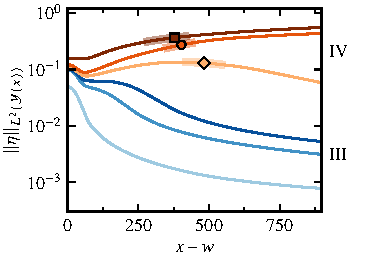
\includegraphics{Images/L2POvsX.pdf}
		\caption{Two-dimensional wave}\label{fig:L2normPOeta}
	\end{subfigure}%
	\begin{subfigure}[b]{0.5\linewidth}
		\centering
		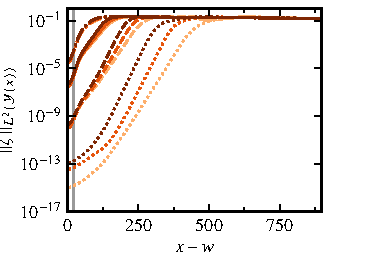
\includegraphics{Images/L2POvsXzeta.pdf}
		\caption{Spanwise perturbation velocity}\label{fig:L2normPOzeta}
	\end{subfigure}\\[6pt]
	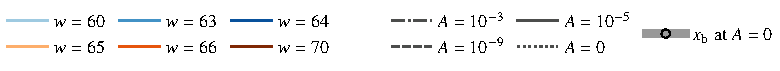
\includegraphics{Images/L2POvsXLegend.pdf}\\[4pt]
	\begin{subfigure}[b]{5.65cm}
		\centering
		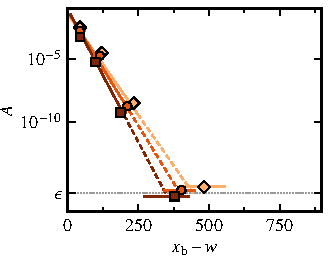
\includegraphics{Images/L2POvsXxb.pdf}
		\caption{Breakdown position}\label{fig:L2normPOxb}
	\end{subfigure}%
	\begin{subfigure}[b]{\dimexpr\linewidth-5.65cm\relax}
		\centering
		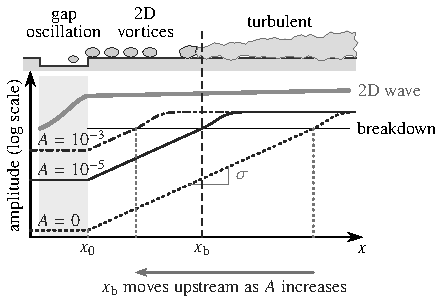
\includegraphics{Images/L2POsketch.pdf}
		\caption{Mechanism}\label{fig:L2normPOsketch}
	\end{subfigure}
	\caption{Streamwise evolution of the self-sustained oscillation and its breakdown for gaps of depth $d=1.5$ at $\Rey=1000$. Colours denote the gap width: blue for widths whose three-dimensional flow returns to the two-dimensional limit cycle (region III), orange for widths whose flow breaks down (region IV). Line styles denote the amplitude $A$ of the forcing~\eqref{eq:seedForcing}. (a) Time-averaged $\|\eta\|_{L^2(\mathcal{Y}(x))}$~\eqref{eq:amplitudeNorm3D} of the two-dimensional limit cycles. Upstream of breakdown the three-dimensional flows coincide with these curves. Markers show the mean breakdown position of the unforced three-dimensional flows, and the shaded segments its range in time. (b) Time-averaged $\|\zeta\|_{L^2(\mathcal{Y}(x))}$ of the three-dimensional flows, once $x_\mathrm{b}$ has stopped drifting. The grey line marks the centre of the forcing. (c) Breakdown position against $A$: mean (markers) and range (bars) of the instantaneous $x_\mathrm{b}$ over the same times. Lines are least-squares fits to the forced simulations, dashed where extrapolated. The unforced simulations, $A=0$, are placed at the machine precision $A=\epsilon$ (dotted line). (d) Sketch of the mechanism: three-dimensional disturbances grow at the rate $\sigma$ from the downstream edge of the gap, $x_0$, on the two-dimensional wave sustained by the gap, and break the flow down at $x_\mathrm{b}$, which moves upstream as their initial level increases~\eqref{eq:breakdownPosition}. The flow sketch corresponds to $A=10^{-5}$.}\label{fig:L2normPO}
\end{figure}

\begin{figure}[ht]
	\centering
	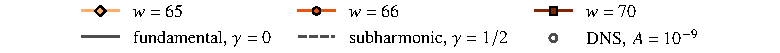
\includegraphics{Images/secStabLegend.pdf}\\[2pt]
	\begin{subfigure}[b]{0.333\linewidth}
		\centering
		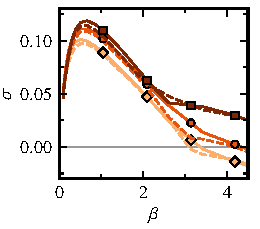
\includegraphics{Images/secStabBeta.pdf}
		\caption{Spanwise wavenumber}\label{fig:secStabBeta}
	\end{subfigure}%
	\begin{subfigure}[b]{0.333\linewidth}
		\centering
		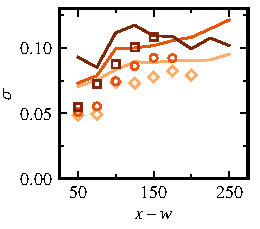
\includegraphics{Images/secStabX.pdf}
		\caption{Streamwise evolution}\label{fig:secStabX}
	\end{subfigure}%
	\begin{subfigure}[b]{0.333\linewidth}
		\centering
		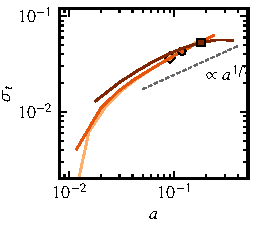
\includegraphics{Images/secStabAmp.pdf}
		\caption{Amplitude of the wave}\label{fig:secStabAmp}
	\end{subfigure}
	\caption{Local secondary stability~\eqref{eq:secondaryEVP} of the two-dimensional waves of the gaps of depth $d=1.5$ at $\Rey=1000$ that break down (region IV). (a) Spatial growth rate $\sigma=\sigma_t/c$ against the spanwise wavenumber at $x-w=150$, for fundamental (solid) and subharmonic (dashed) modes. Markers indicate the wavenumbers $\beta_k=2\pi k/b$ contained in the three-dimensional simulations. (b) Growth rate of the fundamental mode at $\beta_1$ along the wave (lines), and slope of $\|\zeta\|_{L^2(\mathcal{Y}(x))}$ in the simulations forced with $A=10^{-9}$ (open markers), upstream of breakdown. (c) Temporal growth rate of the fundamental mode at $\beta_1$ and $x-w=150$ against the peak amplitude of the fundamental of the wave, $a$, with the wave scaled from its actual amplitude (filled markers).}\label{fig:secStab}
\end{figure}

\bibliographystyle{jfm}
\bibliography{jfm}

\end{document}
